\documentclass[a4paper,norsk,12pt]{book}

\usepackage[norsk]{babel}
\usepackage{enumitem}
\usepackage{color}
\usepackage{amsmath}
\usepackage{wrapfig}
\usepackage{graphicx}
\usepackage[utf8]{inputenc}
\usepackage{hyperref}
\usepackage{icomma}
\usepackage{subcaption}
\usepackage{multirow}
\def\d{\ensuremath{\text{d}}}
\def\half{\ensuremath{\frac{1}{2}}}
\def\ipsqrt{\ensuremath{\frac{1}{\sqrt{2}}}}
\def\imsqrt{\ensuremath{\frac{-1}{\sqrt{2}}}}

\begin{document}
\tableofcontents

\chapter{Introduksjon}
Mot slutten av 1800-tallet var fysikere kommet så langt at det kunne se ut til at man snart hadde oversikt over alle de fundamentale lovmessighetene som styrte naturen. Det har blitt sagt at Lord Kelvin---datidens kanskje mest toneangivende fysiker---uttalte at ``There is nothing new to be discovered in physics now. All that remains is more and more precise measurement.'' Sitatet passer godt inn i den vanlige historiefortellingen om hvordan fysikken utviklet seg, men antakelig sa Lord Kelvin aldri dette. Derimot holdt han en forelesning i Royal Society der han pekte på at to ``skyer på horisonten'' som sto i veien for forståelsen av de underliggende lovmessighetene~\cite{doi:10.1080/14786440109462664}. Den ene skyen var Michelson og Morely sitt forsøk på å måle lysets hastighet gjennom eteren. Forklaringen på deres måleresultat kom gjennom Einstein sin relativitetsteori---et av de to store gjennombruddene tidlig på 1900-tallet som skulle prege fysikkens utvikling videre. Den andre skyen var den såkalte ultrafiolette katastrofen i forbindelse med svart legeme-stråling. Dette problemet fikk sin løsning gjennom kvantemekanikken---det andre av de to store gjennombruddene tidlig på 1900-tallet som skulle prege fysikkens utvikling videre. Denne teksten vil gi en kort innføring i noen aspekter ved kvantemekanikken og se på hvordan dette kan benyttes til å utvide begrepet for hva en datamaskin er og hvordan den kan gjøre beregninger.

\chapter{Kvantemekanikk}

Tidlig i fysikkundervisningen lærer vi at ved å se på summen av krefter på som virker på et objekt kan vi finne ut hvordan det vil bevege seg, $\sum\vec{F} = m\vec{a}$. Hvis vi prøver å bruke denne ligningen til å forutse hvordan et elektron beveger seg vil vi ofte\footnote{Det finnes tilfeller der Newtons lover gir en god beskrivelse av bevegelsen til elektroner, men i det generelle tilfellet er det ikke slik.} få feil resultat. Det viser seg at bevegelsen til elektroner---og andre tilstrekkelig små partikler og systemer av partikler---må beskrives på en helt annen måte. Det er det kvantemekanikken dreier seg om. Denne teksten vil ikke forsøke å gi en fullstendig innføring i kvantemekanikk, men bare diskutere litt generelle aspekter ved kvantemekanikken og gi en litt grundigere diskusjon av de elementene som er nødvendig for å forstå hvordan kvantedatamaskiner virker.

\section{Bølgefunksjonen $\psi$}
\label{sec:kvante:psi}
En kvantemekanisk beskrivelse av verden viser seg å være svært annerledes enn det vi er vant med. Det viser seg at hvis du vil forsøke å forutsi hvilket resultat en måling---for eksempel av posisjonen eller farten til et elektron---vil gi må du nøye deg med å forutsi hvordan sannsynligheten for ulike måleresultater du kan få er. Dette dreier seg ikke om den vanlige måleusikkerheten som skyldes at måleinstrumentet ikke er perfekt, men det er en underliggende fysisk realitet. La oss for konkrethet se på posisjonen til et elektron. I klassisk fysikk som vi kjenner den fra før ville vi benevnt posisjonen med en vektor
\begin{displaymath}
	\vec{r} = (x,y,z)
\end{displaymath}
som beskriver posisjonen til elektronet med tre koordinater som i prinsippet kan bestemmes eksakt. Hvis vi kjenner alle kreftene som virker kan vi beregne hvordan posisjonen varierer med tiden,
\begin{displaymath}
	x = x(t),\quad y = y(t),\quad z=z(t),
\end{displaymath}
slik at vi vet nøyaktig hvor elektronet er også på et vilkårlig tidspunkt i fremtiden.

En kvantemekanisk beskrivelse av elektronet innebærer en såkalt bølge\-funksjon som forteller oss om sannsynligheten for å finne elektronet på et bestemt sted. I det videre vil jeg begrense meg til å beskrive endimensjonal bevegelse for å forenkle notasjonen, men konseptet kan enkelt utvides til tre dimensjoner. Til å beskrive elektronets posisjon bruker vi funksjonen $\psi(x)$, men denne må tolkes på en helt annen måte enn vektoren $\vec{r}$ ovenfor. For det første vil $\psi(x)$ normalt ha en verdi som er ulik null i mer enn ett punkt, noe som betyr at elektronet ikke har en fast definert posisjon, men kan tenkes å være flere steder. Merk at dette faktisk ikke er et uttrykk for at det finnes informasjon om hvor elektronet egentlig er som vi mangler, men at posisjonen til elektronet ikke er fast definert\footnote{Denne bemerkningen fortjener egentlig en lang diskusjon, men dette er ikke stedet for denne diskusjonen. Det er skrevet mye om dette andre steder.}. Figur \ref{fig:kvante:psix} viser to mulige funksjoner $\psi(x)$ som beskriver posisjonen til et elektron som befinner seg ved eller nær $x=1~\mathrm{m}$. Den stiplete blå linjen er kun ulik null i et relativt lite område nær $x=1~\mathrm{m}$. Dette betyr at vi har en ganske stor visshet om hvor elektronet som beskrives av denne $\psi$-funskjonen er. Den heltrukne røde linjen er mer fordelt utover og innebærer derfor at det er et større område der det er sannsynlig at vi vil finne elektronet. 
\begin{figure}[htp]
\begin{center}
	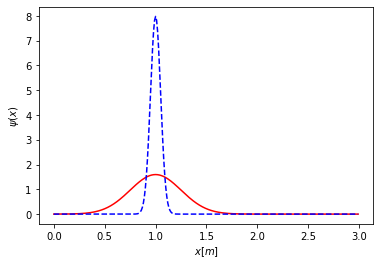
\includegraphics[width=.5\textwidth]{./psix}
	\caption{}
	\label{fig:kvante:psix}
	\end{center}
\end{figure}

Hva skjer så når vi prøver å måle hvor elektronet er? Da vil vi---uansett hvor konsentrert eller utspredt bølgefunksjonen som beskriver det er---finne elektronet lokalisert i ett punkt\footnote{Selvfølgelig med en presisjon som er begrenset av måleinstrumentet vi bruker.}. Dette innebærer at når vi måler hvor elektronet er endrer vi samtidig bølgefunksjonen som beskriver elektronet til å bli mye mer konsentrert rundt ett punkt, men dette punktet trenger ikke nødvendigvis å være der den tidligere hadde maksimum. Det vil imidlertid alltid være et sted der $\psi(x)$ før målingen var ulik null. Hvis vi kjenner bølgefunksjonen før vi måler kan vi bruke den til å beregne sannsynligheten for å finne elektronet i ulike områder. Det gjør vi ved å integrere over kvadratet av absoluttverdien av $\psi(x)$. For eksemel er sannsynligheten for å finne elektronet et sted mellom $x=0,75~\mathrm{m}$ og $x=0,76~\mathrm{m}$
\begin{equation}
	P ( 0,75~\mathrm{m}<x<0,76~\mathrm{m}) = \int_{0,75~\mathrm{m}}^{0,76~\mathrm{m}}|\psi(x)|^2\d x
	\label{eq:kvante:prob}
\end{equation}
Noen bemerkninger om funksjonen $\psi(x)$
\begin{enumerate}
\item
For at integralet i ligning (\ref{eq:kvante:prob}) skal gi en meningsfull sannsynlighet må funksjonen $\psi(x)$ oppfylle et normaliseringskrav, nemlig 
\begin{displaymath}
	1 = \int_{-\infty}^\infty |\psi(x)|^2\d x.
\end{displaymath}
Dette betyr for det første at sannsynligheten for å finne elektronet et eller annet sted er 1. For det andre, siden $|\psi(x)|^2 \geq 0$ overalt vil vi da være sikret å finne sannsynlighet $P\leq1$ dersom vi integrerer over et kortere intervall.
\item
Når vi integrerer over kvadratet av absoluttverdien til funksjonen ($|\psi|^2$) og ikke bare over kvadratet av funksjonen ($\psi^2$) er det fordi det viser seg at vi generelt må tillate $\psi(x)$ å ha komplekse verdier. I enkelte sammenhenger er dette av stor betydning, men i denne teksten får vi ikke behov for å studere dette videre.
\item
Vi har så langt diskutert bølgefunksjonen som en helt vanlig funksjon som tar inn ett tall (posisjonen) og gir ut ett tall (som riktignok kan være komplekst) som kan relateres til sannynligheten for å finne elektronet akkurat der. Generelt vil vi trenge litt mer kompliserte konstruksjoner. En første enkel utvidelse av dette er å ta med de to andre romlige koordinatene samt å ta med en tidsavhengighet som beskriver at bølgefunksjonen endrer seg når tiden går\footnote{En vanlig konvensjon er å bruke stor $\Psi$ for å betegne en bølgefunksjon som avhenger av både rom- og tidskoordinater, mens man bruker liten $\psi$ dersom bølgefunksjonen kun avhenger av de romlige koordinatene, men ikke endrer seg når tiden går.}:
\begin{displaymath}
	\Psi(x,y,z,t).
\end{displaymath}
Videre er det i en del sammenhenger---blant annet en vi skal se på snart og få mye bruk for i resten av denne teksten---ofte nyttig å la bølgefunksjonen gi ut en vektor i stedet for bare et tall:
\begin{displaymath}
	\Psi(x,y,z,t) = \left[ \begin{array}{cc}\phi_1(x,y,z,t) \\ \phi_2(x,y,z,t) \end{array}\right],
\end{displaymath}
der $\phi_1(x,y,z,t)$ og $\phi_2(x,y,z,t)$ er vanlige funksjoner som gir ut (muligens komplekse) tall.
\end{enumerate}

\section{Schr{\"o}dingerligningen}
Gitt en bølgefunksjon $\Psi(x,y,z,t)$ og en funksjon $V(x,y,z)$ som beskriver den potensielle energien som funksjon av posisjonen kan vi finne tidsutviklingen til bølgefunksjonen ved å løse en partiell differensialligning som er kjent som Schr{\"o}dingerligningen (her skrevet opp med bare \'en romlig koordinat):
\begin{displaymath}
	i\hbar\frac{\partial}{\partial t}\Psi(x,t) = \left[ - \frac{\hbar^2}{2m}\frac{\partial^2}{\partial x^2} + V(x)\right]\Psi(x,t)
\end{displaymath}
Her er $m$ massen til partikkelen som beskrives, i vårt tilfelle elektronmassen, og $\hbar = \frac{h}{2\pi} = 1,055\times10^{-34}~\mathrm{Js}$ er den reduserte Planck-konstanten. Schr{\"o}dingerligningen spiller omtrent samme rolle i kvantemekanikken som Newtons andre lov ($\Sigma \vec{F} = m\vec{a}$) spiller i klassisk mekanikk: Den tillater oss å beregne hva som vil skje i fremtiden med kunnskap om hvordan tilstanden er nå. Det er imidlertid noen vesentlige forskjeller. For det første er det bare presisjonen i målingene som begrenser presisjonen i forutsigelsen i klassisk mekanikk. I kvantemekanikk kan vi---som allerede diskutert---kun beregne sannsynligheten for ulike måleresultater, ikke forutsi med sikkerhet hva vi vil måle. Så selv om vi skulle kjenne bølgefunksjonen slik den er nå uten usikkerhet, og dermed kunne forutsi hvordan den vil være i fremtiden uten usikkerhet vil vi fremdeles ikke vite hvilket måleresultat vi ender opp med. For det andre kan Newtons andre lov brukes ``baklengs'': Hvis vi måler hva posisjon og fart er nå kan vi bruke det til å regne ut hva posisjon og fart var på et tidligere tidspunkt. Siden en måling påvirker bølgefunksjonen kan vi ikke bruke Schr{\"o}dingerligningen til å finne ut hvordan bølgefunksjonen var på et tidspunkt før vi målte f.eks. posisjonen til elektronet.

I en generell innføring til kvantemekanikk legges det som regel stor vekt på å løse Schr{\"o}dingerligningen for ulike potensialer $V(x)$. Dette er ikke nødvendig for diskusjonen videre i denne teksten, så det problemet vil ikke bli diskutert videre her.

\section{Spinn}
\label{sec:kvante:spinn}
En del subatomære partikler, inkludert elektronet som vi fokuserer mest på her, har en egenskap som heter spinn. Ordet spinn antyder at det er noe som snurrer rundt, men det er ikke tilfellet. Det er snakk om en iboende egenskap i partikkelen. Likevel kan rotasjonen til en snurrebass være en brukbare analogi for \emph{enkelte aspekter} ved spinnet. Spinn er en vektor som altså har både en størrelse og en retning. I snurrebassanalogien svarer størrelsen til hvor fort den roterer, mens retningen svarer til retningen rotasjonsaksen peker. Positiv retning defineres slik at snurrebassen roterer mot klokken når vi ser den fra den positive siden. Det viser seg at spinnet til subatomære partikler alltid er på formen $\frac{a}{2}\hbar$ der verdien av $a$ avhenger av hvilken partikkel det dreier seg om. Partikler der $a$ er et partall slik at spinnet er et heltall multiplisert med $\hbar$ kalles bosoner. Partikler der $a$ er et oddetall kalles fermioner. Elektronet har $a = 1$ slik at spinnet til elektronet har størrelse $\half\hbar$. Ofte skriver vi dette bare som spinn \half, og jeg vil bruke denne konvensjonen i det videre.

I det videre bryter analogien med en snurrebass fullstendig sammen. I stedet for å måle hvilken retning spinnet til et elektron peker er det enklere å måle projeksjonen av spinnet inn på en vilkårlig akse. Hvis vi gjør dette med en snurrebass vil vi finne en verdi av projeksjonen $s$ slik at  $-S < s < +S$, der $S$ er størrelsen til spinnet. $s=+S$ og $s=-S$ svarer til at aksen vi måler langs er enten parallell eller antiparallell med rotasjonsaksen. $s=0$ svarer til at aksen vi måler langs står normalt på rotasjonsaksen. Når vi gjør denne målingen på et elektron finner vi alltid $+\half$ eller $-\half$ uansett hvilken akse vi måler langs. Sett nå at vi preparerer et elektron med spinnet sitt rettet langs den positive $x$-aksen. Hvis vi nå velger å måle projeksjonen av spinnet på $x$-aksen vil vi med sikkerhet ende opp med resultatet $+\half$. Hvis vi derimot velger å måle projeksjonen av spinnet langs positiv $z$-akse (som står normalt på $x$-aksen) vil vi ende opp med å måle enten $+\half$ eller $-\half$ med 50\% sannsynlighet for hver av verdiene. Hvis vi etter å ha målt projeksjonen langs $z$-aksen igjen måler projeksjonen langs $x$-aksen vil vi ikke lenger med sikkerhet måle $+\half$. Derimot vil vi nå bare ha 50\% sannsynlighet for at målingen viser $+\half$, mens det også er 50\% sannsynlighet for å få verdien $-\half$. 

Som en avslutning av denne første diskusjonen av spinntet tar jeg med at hvis vi igjen preparerer elektronet med spinn opplinjert med $x$-aksen og deretter måler projeksjonen av spinnet på en akse som danner en vinkel $\theta$ med $x$-aksen da blir sannsynlighetene for de to mulige resultatene av målingen
\begin{displaymath}
	P\left(+\half\right) = \cos^2\theta, \quad P\left(-\half\right) = 1- \cos^2\theta = \sin^2\theta.
\end{displaymath}

\section{Måleproblemet}
Både i diskusjonen av posisjonen til elektronet i avsnitt \ref{sec:kvante:psi} og retningen til elektronspinnet i avsnitt \ref{sec:kvante:spinn} var det en underliggende observasjon som ikke ble tydelig formulert:
\begin{quote}
Når vi utfører en måling på et kvantemekanisk system kan vi ikke unngå å samtidig påvirke systemet.
\end{quote}
Dette er helt sentralt, og viser en tydelig forskjell på klassisk mekanikk og kvantemekanikk. I klassisk mekanikk ser vi på objekter som er store nok til at vi kan måle størrelser som for eksempel posisjon eller fart uten relevant påvirkning av størrelsen vi ønsker å måle. Vi kan for eksempel måle posisjonen til en ball ved å \emph{se på den} mens vi har en linjal like ved for å definere måleskalaen. For at vi skal kunne se ballen må det skinne lys på den som reflektres inn i øynene våret. Lyset består av små partikler som kalles fotoner som treffer overflaten til ballen før de sendes videre til, blant annet, øynene våre. Når fotonene treffer ballen gir de den en liten dytt, så i prinsippet kan de endre posisjonen til ballen i prosessen. I praksis er imidlertid bevegelsesmengden til fotonene så liten at de ikke gir noen relevant kraftvirkning på ballen. Derfor kan vi jobbe som om måleprosessen ikke i det hele tatt påvirker det vi ønsker å måle. Dette er ikke tilfellet når vi kommer til kvantemekanikk.

Vi fortsetter å bruke elektronet som eksempel. Massen til et elektron er $m_e = 9,1\times10^{-31}~\mathrm{kg}$. Bevegelsesmengden til et foton avhenger av bølgelengden. Om vi ser på et foton omtrent midt i det synlige spekteret ($\lambda = 550~\mathrm{nm}$) har det bevegelsesmengden $p = \frac{h}{\lambda} = 1,2\times10^{-27}~\mathrm{kg\, m/s}$. Hvis vi bruker dette fotonet til å måle hvor elektronet er vil vi altså samtidig gi elektronet en så kraftig dytt at det etterpå vil ha stor fart bort fra det stedet det var. Slik er det med alle målinger i kvantemekanikken---måleprosessen påvirker systemet vi måler på. Og enda verre, jo mer nøyaktig vi prøver å måle, jo mer vil vi ende opp med å påvirke systemet. Generelt kan vi si at hvis vi ikke kan gjøre målingen på en slik måte at påvirkningen på systemet er neglisjerbar så må vi behandle systemet som kvantemekanisk. Hvis vi derimot kan måle på det uten at målingen gir noen relevant påvirkning på systemet kan vi behandle det med vanlig klassisk mekanikk. 

Det finnes noen spesialtilfeller der vi tilsynelatende unslipper dette måle\-problemet, selv når vi jobber med et system som må behandles kvante\-mekanisk. Et viktig eksempel, og det eneste jeg vil se på her, er gjentatte målinger av elektronspinnet. I avsnitt \ref{sec:kvante:spinn} diskuterte jeg hvordan projeksjonen av spinnet på en akse antar tilfeldige verdier. Men hvis vi repeterer gjentatte målinger langs den samme aksen får vi hele tiden samme resultat. Med andre ord, hvis spinnet er opplinjert med $x$-aksen og vi fortsetter å måle projeksjonen av spinnet inn på $x$-aksen vil ikke målingen endre spinnet. Hvis vi derimot velger å måle spinnet langs en annen akse, for eksempel $z$-aksen, vil målingen påvirke spinnet som diskutert ovenfor.

\chapter{Matriser}

Parallelt med at Erwin Schr\"odinger kom frem til ligningen som jeg nevnte såvidt i forrige kapittel, kom Werner Heisenberg frem til en helt annen matematisk formalisme for å utføre kvantemekaniske beregninger - basert på matriser og vektorer, altså det vi kjenner som lineær algebra. Dette var en gren av matematikken som var ukjent for de fleste fysikere på begynnelsen av 1900-tallet og derfor fikk Heisenberg sin \emph{matrisemekanikk} i første omgang en litt kjøligere mottakelse enn Schr\"odinger sin \emph{bølgemekanikk}. Det viste seg imidlertid at begge formuleringene av kvantemekanikken var like riktig, og at hvilken formulering som var få foretrekke var avhengig av hvilket problem man studerte. Når vi i det videre stort sett skal studere spinnet til elektronet er det Heisenberg sin matrisemekanikk som passer best. Dette kapittelet vil gi en kort repetisjon av lineær algebra og vise hvordan dette brukes til å regne med elektron-spinn.

\section{Basisvektorer}
I et todimensjonalt koordinatsystem trenger vi nøyaktig to tall til å angi en posisjon, vanligvis omtalt som $x$-koordinaten og $y$-koordinaten. Punktet med $x$-koordinat $X$ og y-koordinat $Y$ angis da på vektorform som 
\begin{displaymath}
	\left[\begin{array}{c} X \\ Y \end{array}\right] \text{ eller } \left[X\;Y\right].
\end{displaymath}
Den første formen kaller vi en kolonne-vektor og den andre en rekkevektor. Det er først når vi skal se på multiplikasjon av vektorer med hverandre eller med matriser at forskjellen på disse to representasjonene blir relevant. Akkurat nå kan vi se på de som to likeverdige måte å spesifisere det samme punktet i koordinatsystemet. En litt annen måte å skrive ned den samme informasjonen på er 
\begin{displaymath}
	\left[\begin{array}{c} X \\ Y \end{array}\right] = X\cdot\left[\begin{array}{c} 1 \\ 0 \end{array}\right] + Y\cdot\left[\begin{array}{c} 0 \\ 1 \end{array}\right]
\end{displaymath}
Her er $\left[\begin{array}{c} 1 \\ 0 \end{array}\right]$ en vektor med lengde 1 som peker langs $x$-aksen, mens $\left[\begin{array}{c} 0 \\ 1 \end{array}\right]$ er en vektor med lengde 1 som peker langs $y$-aksen. Denne måten å skrive ned koordinatene på sier enda mer eksplisitt enn den forrige at vi skal gå $X$ skritt langs $x$-aksen og så $Y$ skritt parallelt med $y$-aksen. Vektorene $\left[\begin{array}{c} 1 \\ 0 \end{array}\right]$ og $\left[\begin{array}{c} 0 \\ 1 \end{array}\right]$ er \emph{enhetsvektorer}, og siden alle vektorer i det todimensjonale rommet kan skrives som en lineærkombinasjon av disse to vektorene utgjør de en \emph{basis} for det todimensjonale rommet. 

Valget av basisvektorer er ikke unikt. For det første kan vi skalere vektorene som utgjør basisen med hver sin vilkårlige konstant (ulik 0), og de vil fremdeles være en basis. F.eks. er $\left[\begin{array}{c} -2 \\ 0 \end{array}\right]$ og $\left[\begin{array}{c} 0 \\ 3 \end{array}\right]$ også en basis. Det er heller ikke nødvendig at basisvektorene våre skal være parallelle med $x$- og $y$-aksen. For eksempel vil $\left[\begin{array}{c} 1 \\ 1 \end{array}\right]$ og $\left[\begin{array}{c} 1 \\ -1 \end{array}\right]$ også utgjøre en basis. Generelt vil to vilkårlige vektorer med lengde ulik 0 og som ikke er parallelle med hverandre utgjøre en basis for det todimensjonale rommet. 

I denne teksten vil vi i hovedsak benytte oss av ulike ordnete, ortonormale basiser. Ordnete betyr at vi holder orden på hva som er den første og hva som er den andre basisvektoren. Hvorfor dette er viktig for oss kommer vi tilbake til senere. Ortonormale betyr for det første at basisvektorene står ortogonalt---altså vinkelrett---på hverandre, og for det andre at de er normalisert---altså har lengde 1. 

\section{Multiplikasjon av vektorer}

\section{Bra-ket notasjon}
I de fleste tekster om lineæralgebra symboliseres en vektorstørrelse enten med en pil over symbolet, $\vec{r}$, eller med fet skrift $\mathbf{r}$. Om man har behov for å skille mellom kolonnevektorer og rekkevektorer er det kolonnevektoren som betegnes som nevnt, mens rekkevektoren betegnes som henholdsvis $\vec{r}\,^T$ eller $\mathbf{r}^T$ der $T$ står for \emph{transponert}. I denne teksten vil jeg i stedet bruke en annen notasjon som ble innført av den britiske fysikeren Paul Dirac. Dette er den notasjonen som er mest vanlig å bruke innen kvantemekanikk, men det brukes sjelden i andre sammenhenger (selv om den gjerne kunne vært brukt ellers også). En kolonnevektor betegnes med symbolet $|r\rangle$ og omtales som en \emph{ket}, mens en rekkevektor betegnes med symbolet $\langle r|$ og omtales som en \emph{bra}. 

\subsection{Indreprodukt i bra-ket notasjon}
For å regne ut indreproduktet mellom to vektorer må vi multiplisere en bra-vektor sammen med en ket-vektor slik at vi får en \emph{bracket}. F.eks. gitt $\langle a|$ og $|b\rangle$ betegnes indreproduktet mellom dem med $\langle a|b\rangle$, og dette er en skalar som alltid når vi tar indreprodukt av to vektorer. Merk at det bare er notasjonen som er ny her---indreproduktet regnes ut på den vanlige måten. Hvis f.eks.
\begin{displaymath}
	\langle a | =  [-2\; 4] \text{ og }  |b\rangle =  \left[\begin{array}{c} 3 \\ 1 \end{array}\right],
\end{displaymath}
da er
\begin{displaymath}
\langle a|b\rangle =  [-2\; 4]  \left[\begin{array}{c} 3 \\ 1 \end{array}\right] = (-2)\cdot3 +  4\cdot 1 = -2.
\end{displaymath}

\subsection{Matrise-vektor-produkt i bra-ket notasjon}
Gitt matrisen $M = \left[\begin{array}{cc} 0 & 2 \\ 3 & 1\end{array}\right]$, bra-vektoren $\langle a|=  [-2\; 4]$ og ket-vektoren  $|b\rangle =  \left[\begin{array}{c} 3 \\ 1 \end{array}\right]$. Vi kan da regne ut 
\begin{align*}
	\langle a|M &= [-2 \; 4] \left[\begin{array}{cc} 0 & 2 \\ 3 & 1\end{array}\right] = [12\; 0], \\
	M|b\rangle &=  \left[\begin{array}{cc} 0 & 2 \\ 3 & 1\end{array}\right]\left[\begin{array}{c} 3 \\ 1 \end{array}\right] = \left[\begin{array}{r}  2\\ 10  \end{array}\right], \\
	\langle a|M|b\rangle &= (\langle a|M)|b\rangle = \langle a|(M|b\rangle) =  36.
\end{align*}
$|b\rangle M$ og $M\langle a|$ er derimot ikke definert.

\chapter{Kvantedatamaskiner}

\section{Qubits}

Den grunnleggende informasjonsenheten i vanlige datamaskiner er en \emph{bit}. En bit har enten verdien 0 eller 1 og kan representeres av et hvilket som helst fysisk objekt som har to mulige tilstander. Et enkelt eksempel er en lyspære: Vi kan tilskrive tilstanden `lyset på' verdien 1 og `lyset av' verdien 0. Et eksempel med litt mer teknologisk relevans er en kondensator. Vi kan måle spenningen mellom platene i en kondensator. Hvis spenningen er tilnærmet lik 0 (i praksis under en viss grenseverdi) svarer dette til at bit'en vår har verdi 0. Hvis spenningen er over grenseverdien har bit'en verdien 1. Vi kan endre verdien fra 0 til 1 ved å tilføre kondensatoren ladning, og endre verdien fra 1 til 0 ved å lade ut kondensatoren.

I kvantedatamaskiner er den grunnleggende enheten en \emph{qubit}. En \emph{qubit} er et kvantemekanisk system som har nøyaktig to ulike utfall av en gitt måling. Et typisk eksempel er elektron-spinnet som ble diskutert i avsnitt \ref{sec:kvante:spinn}. Hvis vi måler spinnet langs en gitt akse, f.eks. $x$-aksen, vil vi alltid få enten $+\half$ eller $-\half$. I likhet med den klassiske datamaskinen kan vi tilskrive det ene måleresultatet verdien 1 og det andre måleresultatet 0. Hvis vi leser av verdien til en qubit har den---akkurat som en bit---altså enten verdien 1 eller verdien 0.

Det som virkelig skiller en \emph{qubit} fra en \emph{bit} er hva som skjer med den når vi ikke sjekker hvilke verdi den har. En bit er et klassisk system, og den har den verdien den har inntil vi gjør noe for å endre verdien (eller noe går galt). En qubit derimot er et kvantemekanisk system og må altså beskrives av en bølgefunksjon som diskutert i avsnitt \ref{sec:kvante:psi}. Dette innebærer at vi \emph{kan} sette qubiten til å ha en bestemt verdi som vi kan lese ut igjen senere. For eksempel hvis vi preparerer elektronet vårt slik at det har spinnet rettet i $x$-retning, vil vi finne nettopp at spinnet er rettet i $x$-retning når vi senere måler det. Men vi kan også sette qubiten til å være i en \emph{superposisjon} av de to tilstandene. Som diskutert i avsnitt \ref{sec:kvante:spinn} kan vi preparere elektronet til å ha spinnet sitt i positiv $z$-retning. Hvis da senere måler verdien av spinnet i $x$-retning har vi 50\% sannsynlighet for å få verdien $+\half$ og 50\% sannsynlighet for å få verdien $-\half$. Det er akkurat som om qubiten har både verdien 0 og 1 helt frem til den blir målt, og først da ender opp med den ene eller den andre muligheten. Det er heller ikke nødvendig å la superposisjonen være slik at det er nøyaktig 50\% sannsynlighet for hvert av utfallene. Generelt kan vi ende opp med en vilkårlig fordeling av sannsynligheten på de to ulike utfallene. Det er muligheten for superposisjon mellom de to ulike utfallene som utnyttes i kvantedatamaskiner og som gjør at de kan utføre enkelte beregninger langt raskere enn klassiske datamaskiner. 

\section{Dekoherens}
Så langt har vi diskutert kvantemekaniske systemer som om de er helt stabile. Ta eksempelet med elektronet som vi preparerer med spinnet i positiv $x$-retning. Vi har da sagt at hvis vi måler verdien av spinnet i $x$-retning på et senere tidspunkt (uten å ha gjort noen andre målinger på det i mellomtiden) vil vi nødvendigvis finne at elektronet fremdeles ar spinnet i positiv $x$-retning. Dette er en grov forenkling. Dersom elektronet hadde vært fullstendig isolert fra omgivelsene til enhver tid bortsett fra når vi utfører målingen hadde det vært sant, men dette er selvfølgelig umulig å oppnå. Vi må med andre ord innse at vi har muligheten for at en annen vekselvirkning med omgivelsene enn målingen også påvirker tilstanden til elektronet. Dette fenomenet kalles \emph{dekoherens} og utgjør den sannsynligvis største teknologiske utfordringen når man skal konstruere en kvantedatamaskin. Ofte når kvantedatamaskiner omtales brukes antall qubits---per i dag er det som regel opp til noen få titalls---som et mål på hvor kraftig maskinene er, men uten informasjon om forventet tid før dekoherens ødelegger informasjonen i en qubit er dette ikke tilstrekkelig til å vurdere hvor god kvantedatamaskinen er. 

Siden fokus for denne teksten er mer på prinsippene bak kvantedatamaskiner enn praktisk realisering vil jeg ikke diskutere problemet med koherens videre. Når jeg beskriver algoritmer for kvantedatamaskiner vil jeg derfor beskrive dem som om vi har en maskin der dekoherens ikke er noe problem tilgjengelig. 

\chapter{Kvantekryptografi}

Klassisk kryptografi har en fundamental utfordring: hvordan distribuere krypteringsnøkkelen. Hvis man har en krypteringsnøkkel som er like lang som meldingen er det prinsipielt umulig å bryte koden, men sikkerheten avhenger fremdeles av at man vet at ingen har klart å få tak i nøkkelen. Vet hjelp av kvantemekanisk sammenfiltring kan vi distribuere en nøkkel over et åpent nettverk og forsikre oss om at kun den rette mottakeren har fått nøkkelen. For å se hvordan dette kan gjøres tar vi utgangspunkt i BB84-protokollen som ble funnet opp av Charles Bennett og Gilles Brassard~\cite{bb84}.

Alice ønsker å sende en kodet melding til Bob, men frykter at Eva kan forsøke å fange opp meldingen og dekryptere den. For å hindre Eva i å kunne dekryptere meldingen bruker Alice og Bob sammenfiltrede elektroner til å utveksle kodenøkkelen. Alice preparerer det nødvendige antallet par av av sammenfiltrede elektroner og sender ett fra hvert par til Bob og beholder det andre selv. Både Alice og Bob måler spinnet til alle elektronene ved å på hvert elektron bruke \'en av de to ordnete, ortonormale basisene
\begin{displaymath}
	V = \left\{ \left[\begin{array}{c}1\\0\end{array}\right], \left[\begin{array}{c}1\\0\end{array}\right] \right\} 
	\quad \mathrm{ok} \quad 
	H = \left\{ \left[\begin{array}{c}\ipsqrt\\ \imsqrt\end{array}\right], \left[\begin{array}{c}\ipsqrt\\ \imsqrt\end{array}\right] \right\}.
\end{displaymath}



\chapter{Kvante-logiske porter}

Beregninger i en klassisk datamaskin blir gjort av logiske porter som tar inn en eller flere bit og gir ut en eller flere bit som svar. For eksempel tar en AND-port inn to bit og gir ut svaret 1 dersom begge inn-bitene er 1, ellers gir den ut svaret 0. Tilsvarende blir beregninger i en kvantedatamaskin gjort av kvante-logiske porter som tar inn en eller flere qubit og gir ut en eller flere qubit som svar. Likhetene mellom de to typer datamaskiner er altså store, men vi skal etter hvert se at kombinasjonen av at en qubit kan være i en superposisjon mellom 0 og 1 og at to eller flere qubit kan være sammenfiltret gir kvantedatamaskinen muligheter som går langt utover det klassiske datamaskiner har.

\section{Logiske porter og boolsk algebra}
På grunn av den klare analogien med vanlige logiske porter er det nyttig å ha dette friskt i minne når vi skal studere kvante-logiske porter. Derfor gir jeg et kort overblikk av klassiske logiske porter og hvordan de kan kombineres før jeg introduserer den kvantemekaniske versjonen. 

\subsection{Boolsk algebra}
Matematikken som brukes for å analysere logiske porter\footnote{Ofte brukes begrepet operasjoner i stedet for porter, spesielt når man snakker om boolsk algebra på et mer abstrakt nivå. Det er et en-til-en forhold mellom operasjonene i boolsk algebra og logiske porter anvendt i logiske kretser så distinksjonen mellom operasjoner og porter er ikke viktig.} og nettverk av slike er boolsk algebra. Boolsk algebra er en enkel algebra som opererer på variabler som kun kan ha to mulig verdier: SANT eller USANT. I en datamaskin assosieres SANT med bit-verdien 1 og USANT med bit-verdien 0, og i det videre vil jeg bruke 1 og 0 som de mulige verdiene til de boolske variablene. De grunnleggende regneoperasjonene i den boolske algebraen er:

\subsubsection{NOT (symbol $\neg$)}
NOT er en port/operasjon som tar inn en bit og gir ut en bit. En NOT-port vil alltid endre bit-verdien til det motsatte som vist i sannhetstabellen nedenfor.
\begin{center}
\begin{figure}[h]
\begin{subfigure}{.3\textwidth}
	\begin{tabular}{|c|c|}
	\hline
	$P$ & $\neg P$ \\
	\hline
	0 & 1 \\
	1 & 0 \\
	\hline
	\end{tabular}
\end{subfigure}
\begin{subfigure}{.3\textwidth}
	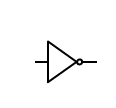
\includegraphics{./gate_not}
\end{subfigure}
\caption{Venstre: Sannhetstabell for NOT-operatoren. Høyre: Kretssymbol for NOT-port.}
\end{figure}
\end{center}

\subsubsection{AND (symbol $\land$)}
AND er en port/operasjon som tar inn to bit og gir ut en bit. AND gir ut 1 dersom begge inn-bitene er 1, ellers gir den ut 0 som vist i sannhetstabellen nedenfor.
\begin{center}
\begin{figure}[h]
\begin{subfigure}{.3\textwidth}
	\begin{tabular}{|c|c|c|}
	\hline
	$P$ & $Q$ & $P \land Q$ \\
	\hline
	0 & 0 & 0\\
	0 & 1 & 0 \\
	1 & 0 & 0 \\
	1 & 1 & 1 \\
	\hline
	\end{tabular}
\end{subfigure}
\begin{subfigure}{.3\textwidth}
	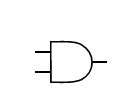
\includegraphics{./gate_and}
\end{subfigure}
\caption{Venstre: Sannhetstabell for AND-operatoren. Høyre: Kretssymbol for AND-port.}
\end{figure}
\end{center}

\subsubsection{OR (symbol $\lor$)}
OR er en port/operasjon som tar inn to bit og gir ut en bit. OR gir ut 1 dersom minst \'en av inn-bitene er 1, ellers gir den ut 0 som vist i sannhetstabellen nedenfor.
\begin{center}
\begin{figure}[h]
\begin{subfigure}{.3\textwidth}
	\begin{tabular}{|c|c|c|}
	\hline
	$P$ & $Q$ & $P \lor Q$ \\
	\hline
	0 & 0 & 0\\
	0 & 1 & 1 \\
	1 & 0 & 1 \\
	1 & 1 & 1 \\
	\hline
	\end{tabular}
\end{subfigure}
\begin{subfigure}{.3\textwidth}
	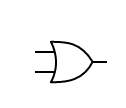
\includegraphics{./gate_or}
\end{subfigure}
\caption{Venstre: Sannhetstabell for OR-operatoren. Høyre: Kretssymbol for OR-port.}
\end{figure}
\end{center}

\subsection{Sammensatte porter}
De ulike portene som er presentert ovenfor kan kombineres til å representere en vilkårlig bineær funksjon\footnote{Det kan vises at det er tilstrekkelig med operasjonene $\neg$ og $\land$ for å oppnå dette, men det er likvel en vanlig konvensjon å beholde $\lor$ på listen over de grunnleggende logiske operasjonene.}, altså en funksjon som tar et antall bit inn og gir ut et antall bit ut med en spesifisert regel for hva som ut verdien(e) blir gitt innverdien(e). Noen slike kombinasjoner er spesielt hyppig brukt og har derfor fått egne navn og symboler. Dette inkluderer:

\subsubsection{XOR (symbol $\oplus$)}
XOR, eller exclucive or, er en operasjon/port som tar inn to bit og gir ut en bit. Denne representerer en enten/eller, altså en port som gir ut verdien 1 hvis \'en, men ikke begge inn-bitene har verdien 1. Ellers gir den ut verdien 0. XOR kan konstrueres som $P\oplus Q = (P\land\neg Q)\lor(\neg P \land Q)$. 
\begin{center}
\begin{figure}[h]
\begin{subfigure}{.3\textwidth}
	\begin{tabular}{|c|c|c|}
	\hline
	$P$ & $Q$ & $P \oplus Q$ \\
	\hline
	0 & 0 & 0\\
	0 & 1 & 1 \\
	1 & 0 & 1 \\
	1 & 1 & 0 \\
	\hline
	\end{tabular}
\end{subfigure}
\begin{subfigure}{.3\textwidth}
	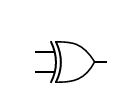
\includegraphics{./gate_xor}
\end{subfigure}
\caption{Venstre: Sannhetstabell for XOR-operatoren. Høyre: Kretssymbol for XOR-port.}
\end{figure}
\end{center}

\subsubsection{NAND (symbol $\uparrow$)}
NAND er en kombinasjon av NOT og AND. Den tar inn to bit og gir ut en bit. Siden NOT er kombinert med AND gir den alltid ut den motsatte verdien av hva AND ville gjort. NAND kan konstrueres som $P \uparrow Q = \neg(P\land Q)$. 

\begin{center}
\begin{figure}[h]
\begin{subfigure}{.3\textwidth}
	\begin{tabular}{|c|c|c|}
	\hline
	$P$ & $Q$ & $P \oplus Q$ \\
	\hline
	0 & 0 & 1\\
	0 & 1 & 1 \\
	1 & 0 & 1 \\
	1 & 1 & 0 \\
	\hline
	\end{tabular}
\end{subfigure}
\begin{subfigure}{.3\textwidth}
	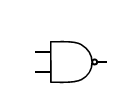
\includegraphics{./gate_nand}
\end{subfigure}
\caption{Venstre: Sannhetstabell for NAND-operatoren. Høyre: Kretssymbol for NAND-port.}
\end{figure}
\end{center}

\subsubsection{CNOT - Controlled NOT}
CNOT er en port som er veldig viktig for oss når vi kommer til kvantedatamaskiner, så derfor tar jeg med beskrivelsen av den klassiske versjonen her. Dette er det første eksempelet vi treffer på av en port med mer enn \'en ut-bit: CNOT tar inn to bit og gir ut to bit. Den første inn-biten ($x$) er kontroll-biten. Verdien av denne biten påvirker hva porten kommer til å gjøre med den andre biten ($y$). I tillegg blir kontroll-biten sendt uforandret ut av porten. Dersom kontroll-biten er 0 vil porten sende den andre biten uforandret ut, mens dersom kontroll-biten er 1 vil porten virke som en NOT-port og altså endre verdien av den andre biten før den sendes ut. Om vi sammenligner med portene som er diskutert ovenfor finner vi at den andre ut-biten bestemmes av en XOR mellom de to innbitene, altså beskrives CNOT av funksjonen $f(x,y) = (x, x\oplus y)$. Effekten av CNOT-porten er oppsummert i sannhetstabellen nedenfor.

CNOT kan konstrueres av en oppsplitting og en XOR-port som vist i figuren nedenfor. Figuren viser også kretssymbolet som vanligvis brukes for CNOT-porter.

\begin{center}
\begin{figure}[h]
\begin{subfigure}{.3\textwidth}
	\begin{tabular}{|c|c||c|c|}
		\hline
	\multicolumn{2}{|c||}{Inn} & \multicolumn{2}{|c|}{Ut} \\
	\hline
	\hline
	$x$ & $y$ & $x$ & $x\oplus y$ \\
	\hline
	\hline
	0 & 0 & 0 & 0 \\
	0 & 1 & 0 & 1 \\
	1 & 0 & 1 & 1 \\
	1 & 1 & 1 & 0 \\
	\hline
	\end{tabular}
\end{subfigure}
\begin{subfigure}{.3\textwidth}
	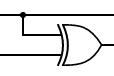
\includegraphics{./gate_cnot_comp}
\end{subfigure}
\begin{subfigure}{.3\textwidth}
	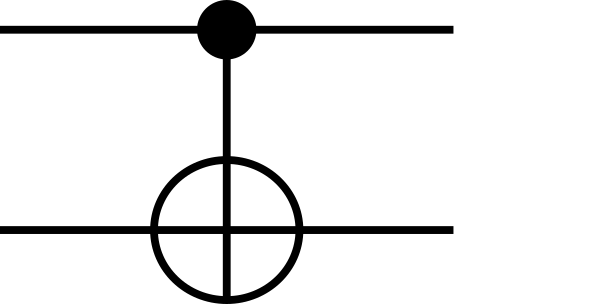
\includegraphics{./gate_cnot}
\end{subfigure}
\caption{Venstre: Sannhetstabell for CNOT-operatoren. Midten: CNOT konstruert med en oppsplitting og en XOR. Øverste inn-bit er $x$ og nederste er $y$. Tilsvarende er øverste ut-bti $x$ og nederste $x\oplus y$. Høyre: Kretssymbol for CNOT-port.}
\end{figure}
\end{center}

CNOT har den interessante egenskapen at den er reversibel. Dette er den fordi det er et en-til-en-forhold mellom hva som blir sendt ut og hva som blir sendt inn. Med andre ord: Hvis vi ser hva som kommer ut er det bare \'en mulighet for hva som ble sendt inn for å produsere dette resultatet. CNOT er dessuten sin egen invers---altså hvis vi lar det som kommer ut av en CNOT-port være innverdiene for den neste kommer vi tilbake til de bit-verdiene vi startet med.

\section{Generalisering til kvante-logiske porter}
For å lage en kvantedatamaskin trenger vi å lage en qubit-versjon av portene som er diskutert ovenfor. Vi støter da straks på en interessant utfordring: mens en klassisk bit alltid er enten 0 eller 1 vil en qubit generelt være i en superposisjon av 0 og 1. Hvordan skal vi lage sannhetstabellene når qubitene har et kontinuerlig sett av mulige verdier? La oss først få på plass litt notasjon som er nyttig i den videre diskusjonen. Nå er det tilstrekkelig for oss å jobbe med \'en basis, og der velger vi $\left\{ \left[\begin{array}{cc}1\\0\end{array}\right], \left[\begin{array}{cc}1\\0\end{array}\right] \right\}$. For å forenkle notasjonen litt kommer jeg for det meste til å skrive vektorene i bra-ket notasjon, med der basisvektorene er identifisert som
\begin{displaymath}
	|0\rangle = \left[\begin{array}{cc}1\\0\end{array}\right] \text{ og } |1\rangle =  \left[\begin{array}{cc}1\\0\end{array}\right].
\end{displaymath}
En generell qubit kan da skrives som $|a\rangle = a_0|0\rangle + a_1|1\rangle$ der $a_0^2 + a_1^2 = 1$. Når vi måler verdien av denne qubiten vil vi finne enten $|0\rangle$ eller $|1\rangle$ med sannynligheter henholdsvis $a_0^2$ og $a_1^2$. Hvis vi har mer enn en qubit å ta hensyn til, må vi ta tensorproduktet av basisvektorene for å finne den nye basisen. For eksempel er basisen for to qubit
\begin{displaymath}
	\left\{ |0\rangle\otimes|0\rangle,  |0\rangle\otimes|1\rangle,  |1\rangle\otimes|0\rangle,  |1\rangle\otimes|1\rangle  \right\}.
\end{displaymath}
For å forenkle notasjonen ytterligere innfører vi konvensjonen at $|00\rangle = |0\rangle\otimes|0\rangle$ og så videre, slik at basisen kan skrives som
\begin{displaymath}
	\left\{ |00\rangle,  |01\rangle,  |10\rangle,  |11\rangle  \right\}.
\end{displaymath}
En generell kombinasjon av to qubit kan da skrives som $|b\rangle = b_{00}|00\rangle + b_{01}|01\rangle + b_{10}|10\rangle + b_{11}|11\rangle$ der $b_{00}^2 + b_{01}^2 + b_{10}^2 + b_{11}^2 = 1$. 

\subsection{Ingen kloning-teoremet}
Vi treffer på en annen viktig forskjell mellom klassisk logikk og kvantelogikk dersom vi ønsker å klone en qubit---det vil si å lage en ekstra kopi av en qubit som er identisk med den vi har. Med klassiske bit er dette ikke noe problem. Hvis vi har en bit med en vilkårlig verdi kan vi uten problemer lage vilkårlig mange kopier av denne. Slik er det ikke i kvanteverden. Det kan vises at i det generelle tilfellet kan man ikke lage en kopi av en qubit slik at man sitter igjen med to qubit som er identiske og lik den vi startet med. Så lenge vi jobber med qubit som har en bestemt verdi er det riktignok ingen forskjell, men for å utnytte oss av fordelene som kan oppnås ved å bruke qubit i superposisjon mellom ulike verdier må algoritmene i en kvantedatamaskin lages på en slik måte at kloning av qubit er unødvendig.

Jeg vil ikke forsøke å bevise ingen kloning-teoremet her, men kun gi kvalitative argumenter som sannsynliggjør at det er riktig. En vilkårlig qubit kan som tidligere beskrevet skrives som $|a\rangle = a_0|0\rangle + a_1|1\rangle$. Dersom vi ønsker å måle verdien av qubiten vil vi aldri få noe annet enn $|0\rangle$ eller $|1\rangle$. Hvis vi kjenner $a_0$ og $a_1$ kan vi riktignok beregne sannsynligheten for hvert av de to ulike måleresultatene, men hva hvis vi har en qubit i en ukjent tilstand? Dersom vi for eksempel får resultatet $|0\rangle$ er det eneste vi kan si om koeffisientene at $a_0>0$. Vi kan altså ikke måle oss frem til hva koeffisientene $a_0$ og$a_1$ er. Men hvis vi ikke kan hente ut denne informasjonen, hvordan kan vi da lage en identisk kopi? 

\bibliographystyle{unsrt}
\bibliography{./referanser}

\end{document}